% Syllabus Template from Arman Shokrollahi
% https://www.overleaf.com/latex/templates/syllabus-template-course-info/gbqbpcdgvxjs

\documentclass[11pt, letterpaper]{article}
%\usepackage{geometry}
\usepackage[inner=2cm,outer=2cm,top=2.5cm,bottom=2.5cm]{geometry}
\pagestyle{empty}
\usepackage{graphicx}
\usepackage{fancyhdr, lastpage, bbding, pmboxdraw}
\usepackage[usenames,dvipsnames]{color}
\definecolor{darkblue}{rgb}{0,0,.6}
\definecolor{darkred}{rgb}{.7,0,0}
\definecolor{darkgreen}{rgb}{0,.6,0}
\definecolor{red}{rgb}{.98,0,0}
\usepackage[colorlinks,pagebackref,pdfusetitle,urlcolor=darkblue,citecolor=darkblue,linkcolor=darkred,bookmarksnumbered,plainpages=false]{hyperref}
\renewcommand{\thefootnote}{\fnsymbol{footnote}}

\pagestyle{fancyplain}
\fancyhf{}
\lhead{ \fancyplain{}{The Science of Cities} }
%\chead{ \fancyplain{}{} }
\rhead{ \fancyplain{}{Fall 2023} }%\today
%\rfoot{\fancyplain{}{page \thepage\ of \pageref{LastPage}}}
\fancyfoot[RO, LE] {page \thepage\ of \pageref{LastPage} }
\thispagestyle{plain}

%%%%%%%%%%%% LISTING %%%
\usepackage{listings}
\usepackage{caption}
\usepackage{setspace}
\DeclareCaptionFont{white}{\color{white}}
\DeclareCaptionFormat{listing}{\colorbox{gray}{\parbox{\textwidth}{#1#2#3}}}
\captionsetup[lstlisting]{format=listing,labelfont=white,textfont=white}
\usepackage{verbatim} % used to display code
\usepackage{fancyvrb}
\usepackage{acronym}
\usepackage{amsthm}
\VerbatimFootnotes % Required, otherwise verbatim does not work in footnotes!



\definecolor{OliveGreen}{cmyk}{0.64,0,0.95,0.40}
\definecolor{CadetBlue}{cmyk}{0.62,0.57,0.23,0}
\definecolor{lightlightgray}{gray}{0.93}



\lstset{
%language=bash,                          % Code langugage
basicstyle=\ttfamily,                   % Code font, Examples: \footnotesize, \ttfamily
keywordstyle=\color{OliveGreen},        % Keywords font ('*' = uppercase)
commentstyle=\color{gray},              % Comments font
numbers=left,                           % Line nums position
numberstyle=\tiny,                      % Line-numbers fonts
stepnumber=1,                           % Step between two line-numbers
numbersep=5pt,                          % How far are line-numbers from code
backgroundcolor=\color{lightlightgray}, % Choose background color
frame=none,                             % A frame around the code
tabsize=2,                              % Default tab size
captionpos=t,                           % Caption-position = bottom
breaklines=true,                        % Automatic line breaking?
breakatwhitespace=false,                % Automatic breaks only at whitespace?
showspaces=false,                       % Dont make spaces visible
showtabs=false,                         % Dont make tabls visible
columns=flexible,                       % Column format
morekeywords={__global__, __device__},  % CUDA specific keywords
}

%%%%%%%%%%%%%%%%%%%%%%%%%%%%%%%%%%%%
\begin{document}
\begin{center}
{\Large \textsc{POLS 4641: The Science of Cities}}
\end{center}
\begin{center}
{\large Fall 2023}
\end{center}

\begin{center}
\rule{6.5in}{0.4pt}
\begin{minipage}[t]{.96\textwidth}
\begin{tabular}{llcccll}
\textbf{Professor:} & Joe Ornstein & & &  & \textbf{Time:} & MWF 12:40pm -- 1:30pm \\
\textbf{Email:} &  \href{mailto:jornstein@uga.edu}{jornstein@uga.edu} & & & & \textbf{Place:} & 101D Baldwin Hall\\
\textbf{Website:} & \href{https://uga.view.usg.edu/d2l/home/2935828}{eLearning Commons (eLC) Course Home} & & & & &
\end{tabular}
\end{minipage}
\rule{6.5in}{0.4pt}
\end{center}
\vspace{.15cm}
\setlength{\unitlength}{1in}
\renewcommand{\arraystretch}{2}

\begin{figure}[h]
	\centering
	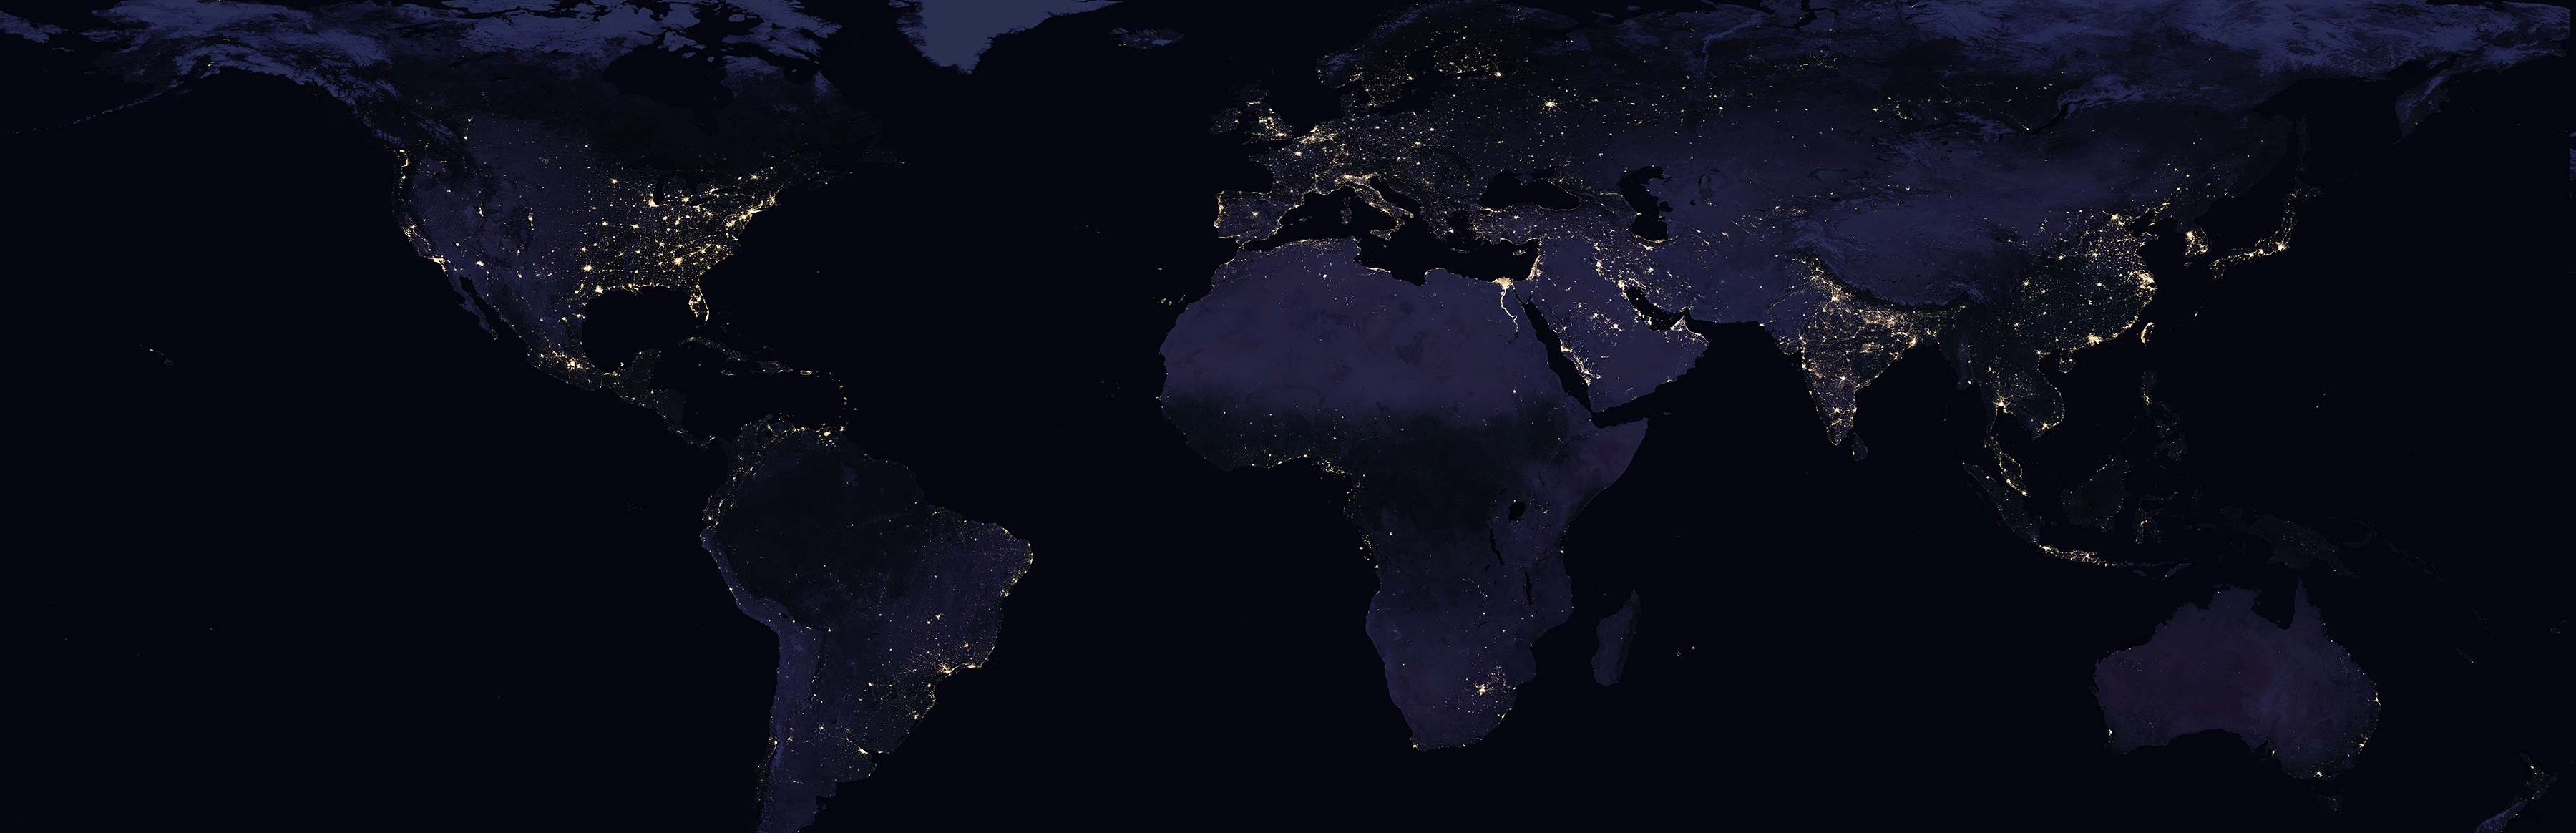
\includegraphics[width = 1.03\textwidth]{img/night-lights-cropped.jpg}
\end{figure}

%\begin{quotation}
%	\noindent``\textit{You can't really know anything if you just remember isolated facts. If the facts don't hang together on a latticework of theory, you don't have them in a usable form. You've got to have models in your head.}''\\
%	\\
%	--Charlie Munger (investor, vice chairman of Berkshire Hathaway)
%\end{quotation}

%% PREAMBLE %%
\onehalfspacing

% Loosely guessed from this: https://www.sciencealert.com/half-the-world-s-population-lives-on-1-of-its-land

\noindent Over half of the Earth's population lives within the sea of city lights visible on the satellite image above. These cities are the centers of global commerce and culture, but in order to function, they require effective governance. Cities need roads, schools, police, fire protection, parks, buses, sewers, and electricity. Many of our most pressing political problems --- including education, transportation, criminal justice reform, housing, and climate change --- are in large part problems of city politics.

In this course, we explore how research from political science, economics, sociology, psychology, and mathematics can help us build cities that are healthier, safer, fairer, and more livable for their residents. The semester will be organized around six modules: foundational research in urban economics, the historical origins of cities, political geography, strengthening local democracy, transportation policy, and housing policy. 

%\section*{Course Objectives}
%%\vskip.15in
%%\noindent\textbf{Course Objectives:}  
%By the end of this course, you will be able to:
%\begin{itemize}
%	\item 
%	\item 
%	\item
%\end{itemize}


\section*{Course Structure}

We will meet three times a week on Mondays, Wednesdays, and Fridays. Each of the course themes will take roughly two weeks to complete; one week for lectures and one week for discussion and review. See our \href{https://uga.view.usg.edu/d2l/home/2935828}{course eLC page} for a more detailed schedule and list of readings. Your grade for the course will be based on four components:

\begin{itemize}
%	\item \textbf{Readings (20\%).} I will assign roughly 2-3 articles/chapters per week. Quiz questions will be drawn from the lectures and these readings, so it will be difficult to perform well without taking time to read the material. I will make the assigned readings available for free on Perusall, where members of the class can mark up the text with questions and comments. To receive full credit, you must spend at least one hour per week reading these assignments. Annotating the texts is encouraged but not required.
	\item \textbf{Quizzes (30 points).} On the final day of each module, we will complete a short (5-10 question, 15 minute) multiple choice quiz through eLC, reviewing the ideas we learned over the past two weeks. You are permitted to reference your notes and course materials during the quiz, but given the short time limit I encourage you not to rely on them.
	\item \textbf{Review Essays (30 points).} Once per module, I will ask you to write a two-page essay (12-point font, double-spaced) explaining 3-5 ideas you've learned, along with 3-5 questions that you would like to discuss during our review periods. These questions can address any topic you choose (e.g. questions about the lectures, readings, general questions about cities). We will use these essays to inform our review sessions before the quizzes. You will receive 5 points per essay completed according to these specifications.
	\item \textbf{Student Presentations (20 points).} Once during the semester, you will deliver an in-class presentation in which you tell a true story meant to illustrate a concept or idea from class. These presentations must adhere to the ``\href{https://en.wikipedia.org/wiki/PechaKucha}{PechaKucha}'' style: twenty slides displayed for twenty seconds each (mostly images, no more than twenty words per slide). The purpose of this assignment is to give you practice explaining some of the ideas we learn, and to recognize them when they appear ``in the wild''. (If you are struggling to find story ideas for your presentation, I have a large number of links to readings and media on a previous version of the \href{https://joeornstein.github.io/pols-4641/}{course website} that may help.) I will grade these presentations according to the following rubric:
	\begin{itemize}
		\item The presentation is engaging and adheres to the required format (5 points).
		\item The story you tell clearly and accurately illustrates a concept from the class (5 points).
		\item Your story's \textit{thesis statement} -- the idea you're trying to communicate -- could be easily summed up in a sentence or two. This thesis statement is clearly presented and relevant to the ideas we discussed in class (5 points).
		\item You have provided sufficient evidence to convince a skeptical audience that your thesis has merit (5 points).
	\end{itemize}
	To sign up for a presentation slot, follow this link to the \href{https://docs.google.com/spreadsheets/d/12a5mE-qxsg_m47bSt2t3PnnQu6zLRQ9DePzw3ObePRc/edit?usp=sharing}{Google Sheet}.
	
	\item \textbf{Final Exam (20 points).} There will be a final exam consisting of short answer and essay questions during our \href{https://reg.uga.edu/general-information/calendars/final-exam-schedule/}{scheduled final exam period}.
\end{itemize}

\noindent At the end of the semester, I will convert your numeric grade to a final letter grade according to the following scale: 93-100 (A), 90-92 (A-), 87-89 (B+), 83-86 (B), 80-82 (B-), 77-79 (C+), 73-76 (C), 70-72 (C-), below 70 (F).

\section*{Office Hours}

I hold office hours by appointment in Baldwin 304C, and you can sign up for 20 minute slots using \href{https://calendly.com/joeornstein/20min}{this link}. I strongly encourage you to sign up for office hours before your presentation so we can discuss any questions you have. Even if you don't have any questions about the material, stop by office hours anyway! One of the great things about college is that your professors are all required to set aside time each week just to talk with their students. And, not to brag, but I'm \textit{pretty good at talking}. My job title (Assistant Professor) is basically just Latin for ``Assistant Talker''.


\section*{Academic Honesty}

Remember that when you joined the University of Georgia community, you agreed to abide by a code of conduct outlined in the academic honesty policy called \href{https://honesty.uga.edu/Academic-Honesty-Policy/Introduction/}{\textit{A Culture of Honesty}}. It has some pretty specific things to say on the subject of cheating. Quite specific. Presentations must be your own original creations, and I will report any and all dishonest conduct to the Office of the Vice President for Instruction. If you use tools such as ChatGPT to generate text or images for your assignments, you must inform the professor and note which parts of the text were the model's contribution. Any other use of such software to disguise plagiarized work is considered unauthorized assistance.

\section*{Mental Health and Wellness Resources}

\begin{itemize}
\item If you or someone you know needs assistance, you are encouraged to contact Student Care and Outreach in the Division of Student Affairs at 706-542-7774 or visit \href{https://sco.uga.edu}{https://sco.uga.edu}. They will help you navigate any difficult circumstances you may be facing by connecting you with the appropriate resources or services. 
\item UGA has several resources for a student seeking \href{https://www.uhs.uga.edu/bewelluga/bewelluga}{mental health services} or \href{https://www.uhs.uga.edu/info/emergencies}{crisis support}. 
\item If you need help managing stress anxiety, relationships, etc., please visit \href{https://www.uhs.uga.edu/bewelluga/bewelluga}{BeWellUGA} for a list of FREE workshops, classes, mentoring, and health coaching led by licensed clinicians and health educators in the University Health Center.
\item Additional resources can be accessed through the UGA App.
\end{itemize}



%%%%%% THE END 
\end{document} 